%%% Exemplo de utilização da classe ITA
%%%
%%%   por        Fábio Fagundes Silveira   -  ffs [at] ita [dot] br
%%%              Benedito C. O. Maciel     -  bcmaciel [at] ita [dot] br
%%%              Giovani Volnei Meinertz   -  giovani [at] ita [dot] br
%%%    	         Hudson Alberto Bode       -  bode [at] ita [dot]br
%%%    	         P. I. Braga de Queiroz    -  pi [at] ita [dot] br
%%%    	         Jorge A. B. Gripp         -  gripp [at] ita [dot] br
%%%    	         Juliano Monte-Mor         -  jamontemor [at] yahoo [dot] com [dot] br
%%%    	         Tarcisio A. B. Gripp      -  tarcisio.gripp [at] gmail [dot] com
%%%
%%%   Versão para overleaf:
%%%   por           Alejandro A. Rios Cruz - aarc.88@gmail.com
%%%                 Saulo Gómez            - sagomezs@unal.edu.co
%%%  IMPORTANTE: O texto contido neste exemplo nao significa absolutamente nada.  :-)
%%%              O intuito aqui eh demonstrar os comandos criados na classe e suas
%%%              respectivas utilizacoes.
%%%
%%%  Tese.tex  2016-08-25
%%%  $HeadURL: http://www.apgita.org.br/apgita/teses-e-latex.php $
%%%
%%% ITALUS
%%% Instituto Tecnológico de Aeronáutica --- ITA, Sao Jose dos Campos, Brasil
%%%                   http://groups.yahoo.com/group/italus/
%%% Discussion list: italus {at} yahoogroups.com
%%%
%++++++++++++++++++++++++++++++++++++++++++++++++++++++++++++++++++++++++++++++
% Para alterar o TIPO DE DOCUMENTO, preencher a linha abaixo \documentclass[?]{?}
%   \documentclass[tg]{ita}			= Trabalho de Graduacao
%   \documentclass[tgfem]{ita}	= Para Engenheiras
%   								msc     		= Dissertacao de Mestrado
%   								mscfem   		= Para Mestras
%   								dsc      		= Tese de Doutorado
%   								dscfem   		= Para Doutoras
%   								quali    		= Exame de Qualificacao
%   								qualifem 		= Exame de Qualificacao para Doutoras
% Para 'Draft Version'/'Versao Preliminar' com data no rodape, adicionar 'dv':
%   \documentclass[dsc, dv]{ita}
% Para trabalhos em Inglês, adicionar 'eng':
%   \documentclass[dsc, eng]{ita}
%		\documentclass[dsc, eng, dv]{ita}
%++++++++++++++++++++++++++++++++++++++++++++++++++++++++++++++++++++++++++++++
\documentclass[tg, eng]{ita}    % ITA.cls based on standard book.cls
% Quando alterar a classe, por exemplo de [msc] para [msc, eng]) rode mais uma vez o botão BUILD OUTPUT caso haja erro
\usepackage[utf8]{inputenc}
\usepackage{ae}
\usepackage{graphicx}
\usepackage{epsfig}
\usepackage{amsmath}
\usepackage{amssymb}
\usepackage{subfig}
\usepackage{multirow}
\usepackage{float}
\usepackage{amsthm}
\usepackage{url}         % formats URL addresses properly
\usepackage{appendix}    % allows appendix section to be included
\usepackage{lscape}      % allows a page to be rendered in landscape mode
\usepackage{multicol}    % allows text in multi columns
\usepackage{cancel}      % needed to show canceled terms in equations
\usepackage{lettrine}
\usepackage{float}
\usepackage{placeins}


%HHHHHHHHHHHHHHHHHHHHHHHHHHHHHHHHHHHHHHHHHHHHHHHHHHHHHHHHHHHHHHHHHHHHHHHHHHHHHHHHHHHHHHHHHHHHHHHHHHHHHHHHHHHH
%\usepackage{subfigure}
%\usepackage{subfigmat}
%PACOTEFIGURAS_SE _ERRADO_ESXCLUIR_ACIMA
\usepackage{booktabs}
%PACOTETABELAS_SE _ERRADO_ESXCLUIR_ACIMA
%HHHHHHHHHHHHHHHHHHHHHHHHHHHHHHHHHHHHHHHHHHHHHHHHHHHHHHHHHHHHHHHHHHHHHHHHHHHHHHHHHHHHHHHHHHHHHHHHHHHHHHHHHHHH

%++++++++++++++++++++++++++++++++++++++++++++++++++++++++++++++++++++++++++++++
% Espaçamento padrão de todo o documento
%++++++++++++++++++++++++++++++++++++++++++++++++++++++++++++++++++++++++++++++
\onehalfspacing

%singlespacing Para um espaçamento simples
%onehalfspacing Para um espaçamento de 1,5
%doublespacing Para um espaçamento duplo

%++++++++++++++++++++++++++++++++++++++++++++++++++++++++++++++++++++++++++++++
% Identificacoes (se o trabalho for em inglês, insira os dados em inglês)
% Para entradas abreviadas de Professora (Profa.) em português escreva: Prof$^\textnormal{a}$.
%++++++++++++++++++++++++++++++++++++++++++++++++++++++++++++++++++++++++++++++
\course{Computer Engineering}  % Programa de PG ou Curso de Graduação
%\area{Aircraft Design} % Área de concentração na PG (Não utilizado no caso de TG)

% Autor do trabalho: Nome Sobrenome
\authorgender{masc}                     %sexo: masc ou fem
\author{Gabriel}{Barbosa Martinz}
\itaauthoraddress{Rua H8B, 203}{12.228-461}{São José dos Campos--SP}

% Titulo da Tese/Dissertação
\title{Use of generative neural networks for instance space codification and generation of data with specific properties}

% Orientador
\advisorgender{fem}                    % masc ou fem
\advisor{Prof$^\textnormal{a}$.~Dr$^\textnormal{a}$.}{Ana Carolina Lorena}{ITA}

% Coorientador (Caso não haja coorientador, colocar ambas as variáveis \coadvisorgender e \coadvisor comentadas, com um % na frente)
% \coadvisorgender{fem}									% masc ou fem
% \coadvisor{Prof$^\textnormal{a}$.~Dr$^\textnormal{a}$.}{Doralice Serra}{OVNI}

% Pró-reitor da Pós-graduação
\bossgender{masc}												% masc ou fem
\boss{Prof.~Dr.}{Flávio}

%Coordenador do curso no caso de TG
\bosscoursegender{masc}									% masc ou fem
\bosscourse{Prof.~Dr.}{Marcos Máximo}

% Palavras-Chaves informadas pela Biblioteca -> utilizada na CIP
\kwcip{Neural networks}
\kwcip{Instance space}
\kwcip{GAN}

% membros da banca examinadora

\examiner{Prof. Dr.}{Alan Turing}{Presidente}{ITA}
\examiner{Prof. Dr.}{Linus Torwald}{}{UXXX}
\examiner{Prof. Dr.}{Richard Stallman}{}{UYYY}
\examiner{Prof. Dr.}{Donald Duck}{}{DYSNEY}
\examiner{Prof. Dr.}{Mickey Mouse}{}{DISNEY}

% Data da defesa (mês em maiúsculo, se trabalho em inglês, e minúsculo se trabalho em português)
\date{23}{June}{2023}

% Número CDU - (somente para TG)
\cdu{621.38}

% Glossario
\makeglossary
\frontmatter

\begin{document}
% Folha de Rosto e Capa para o caso do TG
\maketitle

% Dedicatoria: Nao esqueca essa secao  ... :-)
\begin{itadedication}
Aos amigos da Graduação do ITA por motivarem tanto a criação deste template pelo Fábio Fagundes Silveira quanto por motivarem a mim e outras pessoas a atualizarem e aprimorarem este excelente trabalho.
\end{itadedication}

% Agradecimentos
\begin{itathanks}
To my parents, Michelle and Raimundo, for always supporting me in my academic journey. To my advisor, Prof. Ana Carolina Lorena for the guidance provided over this research. To my beloved Vitória, for the love and emotional support she gives to me. To my roommates over these years for being great friends. To the friends I've made when at ITA and before it for helping me and making my undergraduate journey more fun. To all the amazing professors I had over my undergraduate studies for shaping my interests in engineering.

\end{itathanks}

% Epígrafe
\thispagestyle{empty}
\ifhyperref\pdfbookmark[0]{\nameepigraphe}{epigrafe}\fi
\begin{flushright}
\begin{spacing}{1}
\mbox{}\vfill
{\sffamily\itshape
``If I have seen farther than others,\\
it is because I stood on the shoulders of giants.''\\}
--- \textsc{Sir~Isaac Newton}

\end{spacing}
\end{flushright}

% Resumo
%\begin{abstract}
%\noindent
%Aqui começa o resumo do referido trabalho. Não tenho a menor idéia do que colocar aqui. Sendo assim, vou inventar. Lá vai: Este trabalho apresenta uma metodologia de controle de posição das juntas passivas de um manipulador subatuado de uma maneira subótima. O termo subatuado se refere ao fato de que nem todas as juntas ou graus de liberdade do sistema são equipados com atuadores, o que ocorre na prática devido a falhas ou como resultado de projeto. As juntas passivas de manipuladores desse tipo são indiretamente controladas pelo movimento das juntas ativas usando as características de acoplamento da dinâmica de manipuladores. A utilização de redundância de atuação das juntas ativas permite a minimização de alguns critérios, como consumo de energia, por exemplo.
Apesar da estrutura cinemática de manipuladores subatuados ser idêntica a do totalmente atuado, em geral suas caraterísticas dinâmicas diferem devido a presença de juntas passivas. Assim, apresentamos a modelagem dinâmica de um manipulador subatuado e o conceito de índice de acoplamento. Este índice é utilizado na sequência de controle ótimo do \mbox{manipulador}.
A hipótese de que o número de juntas ativas seja maior que o número de
passivas  $(n_{a} > n_{p})$  permite o controle ótimo das juntas passivas, uma vez que na etapa de controle destas há mais entradas (torques nos atuadores das juntas ativas), que elementos a controlar (posição das juntas passivas). 
%\end{abstract}

% Abstract
\begin{englishabstract}
\noindent
One topic of study in Machine Learning is the study of algorithmic performance and which methodologies may be used to assess this performance. A methodology known as Instance Space Analysis has been used to relate predictive performance in classification algorithms to instance hardness measures able to assess how hard an instance is for an algorithm to classify. The original methodology has been defined with the instance being an entire dataset, but further work has been made to make the instance as fine-grained as an individual observation. In this work we will build upon this methodology and we propose the creation of a encoder-decoder network model to generate new observations for a classification algorithm with predefined hardness properties.

\end{englishabstract}

% Lista de figuras
\listoffigures %opcional

% Lista de tabelas
\listoftables %opcional

% Lista de abreviaturas
\listofabbreviations
\begin{longtable}{ll}
CTq & computed torque \\
DC & direct current \\
EAR & Equação Algébrica de Riccati \\
GDL & graus de liberdade \\
ISR & interrupção de serviço e rotina \\
LMI & linear matrices inequalities \\
MIMO & multiple input multiple output \\
PD & proporcional derivativo \\
PID & proporcional integrativo derivativo \\
PTP & point to point \\
UARMII & Underactuated Robot Manipulator II \\
VSC & variable structure control \\

\end{longtable}

 %opcional

% Lista de simbolos
\listofsymbol


 %opcional

% Sumario
\tableofcontents


\mainmatter
% Os capitulos comecam aqui

\chapter{Introdução}
\section{Motivation}
Often in a problem being tackled with Machine Learning (ML) techniques one of the most important part of the solving process is the algorithm selection. Each algorithm has a specific bias which makes it more suitable for some classes of problems than others \cite{Adam2019}. 

It is desirable, then, that we may have a way of measuring the relationship of the performance of a given algorithm in a problem with the problem's characteristics, since knowing which data is easy or difficult for a given model to classify is useful in the way that we may make changes to the original model.

\citeonline{Munoz2018} has introduced a methodology called Instance Space Analysis (ISA), a novel way of performance evaluation and algorithm selection in classification problems by mapping the statistical properties of an instance (an entire dataset) into how difficult the instance is for the classification algorithm to perform. Further, in \citeonline{Lorena2022}, the methodology has been modified to have a more fine-grained analysis, with the instance being reduced to an individual observation in a classification dataset.

Given this, we can map each observation into a hardness level. But one feature of the ISA not investigated in the instance-level proposal of \citeonline{Lorena2022} is how to generate new problem instances with desired characteristics in order to expand the dataset with instances that may defy the classification techniques. This project aims to fill this gap. 

One type of model that may give us this feature from this data is a Generative Adversarial Network (GAN) architecture, as defined by \citeonline{Goodfellow2014}. This architecture is based on a zero-sum game, with a generator network trying to create data matching the original data and a discriminator network trying to discern between the original data and the generated data. 

Using this approach, we can use the trained generator to create data with specific hardness levels and be able to challenge the classification techniques at different levels. We can use this to verify how the original model behaves with data with a given difficulty profile or to challenge the model, such as generating adversarial examples \cite{Yuan2019}.

\section{Objective}

This work's objective lies in providing a framework for data generation based on the relationship between instance hardness and classification performance using the GAN architecture and monitor the original model's behaviour using the generated data. 

\section{Scope}

The scope of this work will be limited to exploring a GAN implementation for the generation of data, creating a Generator and a Discriminator.  The modelling will be made entirely using Python, with the PyTorch \cite{paszke2019pytorch} framework. PyHard \cite{Lorena2022} will be used for reproducing the ISA methodology.

%\begin{figure}[ht]
%\centering
%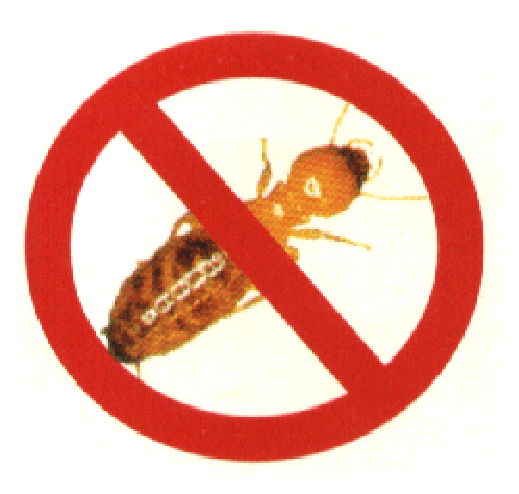
\includegraphics[width=0.5\textwidth]{Cap1/cupim}
%\caption{Proibido estacionar cupins. Legenda grande, com o objetivo de demonstrar a indentação na lista de figuras.}
%\label{cupim}
%\end{figure}


%\begin{figure}[ht!]
%\centering
%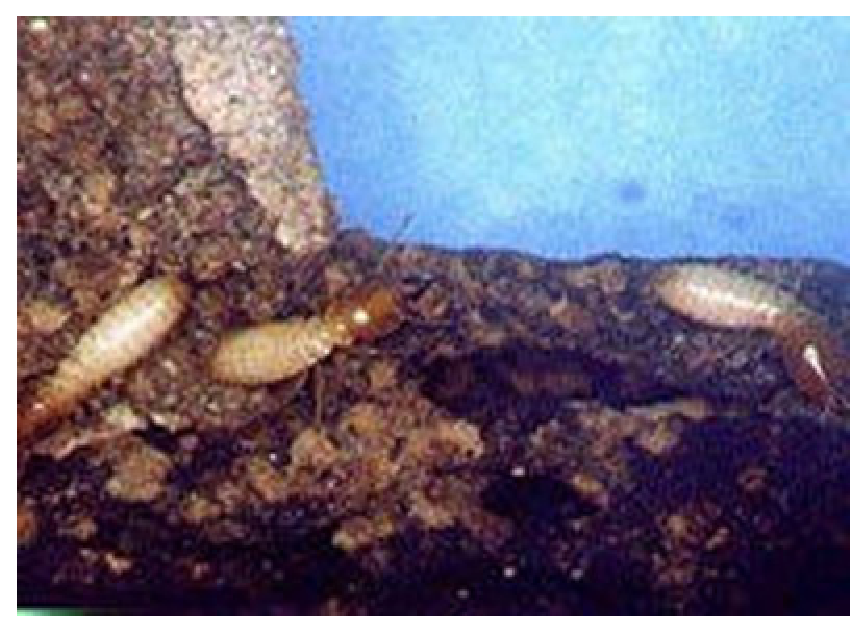
\includegraphics[width=1\textwidth]{Cap1/cupimconcreto}
%\caption{Exemplo real de cupim frente ao seu dilema.}
%\label{FDII}
%\end{figure}

\section{Outline of this work}

The document is organized as follows:

\begin{itemize}
	\item Chapter \ref{ch:machinelearning}  introduces some Machine Learning terminology and describes the GAN neural network model;
	\item Chapter \ref{ch:isa} describes the ISA framework;
	\item Chapter \ref{ch:methodology} presents the methodology to be followed in the computational experiments;
	\item Chapter \ref{ch:conclusion} concludes the work presenting future activities and a work schedule.
\end{itemize}


\chapter{Modelagem Dinâmica de Cupins Cibernéticos}
\section{Instance Space Analysis}
Manipuladores subatuados diferem dos totalmente atuados pois são equipados com um número de atuadores que é sempre menor que o número de graus de liberdade (GDL). Portanto, nem todos os GDL podem ser controlados ativamente ao mesmo tempo \cite{Sbornian2004}. Por exemplo, com um manipulador planar de 3 juntas equipado com dois atuadores, ou seja, duas juntas ativas e
uma passiva, pode-se controlar ao mesmo tempo duas das juntas a qualquer instante, mas não todas. Para controlar todas as juntas de um manipulador subatuado, deve-se usar um controle sequencial. Este princípio foi provado pela primeira vez por {arai} usando  argumentos dinâmicos linearizados \cite{Joea2003}, e é a base para a modelagem no espaço das juntas e no espaço Cartesiano. A Tabela \ref{minhatab} apresenta os resultados \cite{Assenmacher1993,Silberschatz1991,Munoz2018}.

\begin{table}
\caption{Exemplo de uma Tabela}
\label{minhatab}

\center
\begin{tabular}{cccc}
  % after \\: \hline or \cline{col1-col2} \cline{col3-col4} ...
  \hline
	Parâmetro & Unidade & Valor da simulação & Valor experimental   \\
	\hline
  Comprimento, $\alpha$ & $m$ &  $8,23$  & $8,54$ \\
  Altura, $\beta$ & $m$     &  $29,1$ & $28,3$\\
	Velocidade, $v$ & $m/s$  &  $60,2$ & $67,3$\\
	\hline
\end{tabular}
\end{table}

Devido ao fato de que no máximo $n_{a}$ coordenadas generalizadas (ângulos das juntas ou variáveis cartesianas) podem ser controladas num dado instante, o vetor de coordenadas generalizadas é dividido em duas partes, representando as coordenadas generalizadas ativas e as coordenadas generalizadas passivas \cite{Callaghan1995}.

Considerando um robô manipulador rígido, malha aberta, e de $n$-juntas em série. Seja $q$ a representação de seu vetor de posição angular das juntas  e $\tau$ a representação de seu vetor de torque. A equação dinâmica pelo método de
Lagrange é dada por:
\begin{equation} \label{eq:lagr1}
\frac{d}{dt}(\frac{\partial L}{\partial \dot{q}})-\frac{\partial L}{\partial q}=\tau^{T}.
\end{equation}
O Lagrangiano $L$ é definido como a diferença entre as energias cinética e potencial do sistema:
\begin{equation} \label{L}
L=T-P
\end{equation}

A energia cinética total dos ligamentos é representada:
\begin{equation} \label{energT}
T=\frac{1}{2}\dot{q}^{T}M(q)\dot{q}
\end{equation}


\chapter{Controle Robusto de Concretos Caóticos}
In this chapter we will be introducing the novel methodology for algorithm selection and performance evaluation called Instance Space Analysis (ISA), introduced in \citeonline{Munoz2018}. We will be showing the original definition of an instance space and the adaptation of the methodology brought up by \citeonline{Lorena2022} relating instance hardness.

\section{Instance spaces}

ISA is, at its core, an extension of the Algorithm Selection Problem (ASP) \cite{RICE1976}. Figure \ref{fig:ISA_flowchart} shows the ISA framework with the ASP highlighted in blue. The objective in the ASP is to automate the process of selecting algorithms based on past similar solved problems. The following sets compose the core of the ASP:

\begin{itemize}
	\item \textbf{Problem Space} $\mathcal{P}$: contains all instances of the problem being analysed;
	\item \textbf{Instance Sub-space} $\mathcal{I}$: contains a subset of instances from $\mathcal{P}$ for which the characteristics and solutions are available;
	\item \textbf{Feature Space} $\mathcal{F}$: a set of descriptive characteristics of the instances in $\mathcal{I}$. These are also known as meta-features;
	\item \textbf{Algorithm Space} $\mathcal{A}$: contains algorithms that may be used to solve the instances in $\mathcal{I}$;
	\item \textbf{Performance Space} $\mathcal{Y}$: contains the performance evaluations of the algorithms in $\mathcal{A}$ over the instances in $\mathcal{I}$.
\end{itemize}

\begin{figure}[ht]
	\centering
	\begin{tikzpicture}[node distance=4cm]
		
		% Nodes
		\node[rectangle, draw, align=center] (problem) {Problem Space \\ $z \in \mathcal{P}$};
		\node[rectangle, draw, below of=problem, align=center] (subspace) {$x \in \mathcal{I} \subset \mathcal{P}$ \\ Sub-space of \\ instances};
		\node[rectangle, draw, below of=subspace, align=center] (feature) {$f(x) \in \mathcal{F}$ \\ Feature \\ Space};
		\node[rectangle, draw, below of=feature, align=center] (instance) {$g(f(x)) \in \mathbb{R}^2$ \\ 2-D Instance \\ Space};
		\node[rectangle, draw, right of=feature, xshift=4cm, align=center] (algorithm) {$\alpha \in \mathcal{A}$ \\ Algorithm \\ Space};
		\node[rectangle, draw, above of=algorithm, align=center] (performance) {$y \in \mathcal{Y}$ \\ Performance \\ Space};
		\node[rectangle, draw, above of=performance, align=center] (footprints) {Footprints in \\ Instance Space};
		
		% Rectangle
		\begin{scope}[on background layer]
			\node[fill=blue!30, rounded corners, opacity=0.3, fit=(subspace)(feature)(algorithm)(performance), inner ysep=0.5cm, inner xsep=2.5cm] (rectangle) {};
		\end{scope}
		
		% Arrows
		\draw[->] (problem) -- node[left, align=right] {Instance selection\\or generation} (subspace);
		\draw[->] (subspace) -- node[left, align=center] {Feature selection\\$f$} (feature);
		\draw[->] (feature) -- node[left, align=right] {Dimension reduction\\and visualization} (instance);
		\draw[->] (feature) -- node[above] (alpha) {$\alpha^* = S(f(x))$} (algorithm);
		\draw[->] (instance) -| node[above, near start, align=center] {Learn selection\\mapping\\from features} node[below, near start] {$\alpha^* = S^\prime(f(x))$} ++(8cm,0) |-  (algorithm.south);
		\draw[->] (algorithm) -- node[right, align=left] {$y(\alpha, x)$ apply \\algorithm $\alpha$ \\to instance $x$} (performance);
		\draw[->] (performance) -| node[above, near start, align=center] {Select $\alpha^*$ to\\ maximize $||y||$} ++(-4cm,0) |-  (alpha.north);
		\draw[->] (footprints) -- node[above, align=center] {Infer algorithm \\performance on \\all $z \in \mathcal{P}$} (problem);
		\draw[->] (performance) -- node[right, align=left] {Define algorithm \\footprints $\varphi(y(\alpha, x))$} (footprints);
		
	\end{tikzpicture}
	\caption{ISA framework. Extracted from \citeonline{Munoz2018}. The ASP is highlighted in blue.} \label{fig:ISA_flowchart}
\end{figure}

The combination of tuples $(x, f(x), \alpha, y(\alpha, x))$, where $x \in \mathcal{I}$, $f(x) \in \mathcal{F}$, $\alpha \in \mathcal{A}$ and $y(\alpha, x) \in \mathcal{Y}$, composes a meta-dataset $\mathcal{M}$. A meta-learner $S$ can then be trained to select the best algorithm for an instance $x$ based on its meta-features, that is, an algorithm $\alpha^*$ with maximum predictive performance for $x$ as given by $y$: 

\begin{equation} \label{eq:algo_selection}
	\alpha^* = S(f(x)) = \arg \max_{\alpha} ||y(\alpha, x)||.
\end{equation}

The ISA framework goes further to give insights into why some instances are harder to solve than others, using both the information of meta-features and algorithmic performance in a 2-D embedding, called Instance Space (IS), that can be visually inspected. An optimization problem is solved to find the mapping from meta-features to the IS $g(f(x))$, such that the distribution of algorithmic performance metrics and meta-features values display as close a linear trend as possible in the IS embedding. This embedding can then be inspected for regions of good and bad algorithmic performance and a new learner can be created to select new algorithms, as in:

\begin{equation}
	\alpha^* = S^\prime(g(f(x)))
\end{equation}

In the IS, it is also possible to define algorithm footprints $\varphi(y(\alpha, x))$, which are areas where an algorithm $\alpha$ is expected to perform well. A set of objective measures can be derived from these footprints and aid in the inference of algorithmic performance for other instances that were not in $\mathcal{I}$, such as: 

\begin{itemize}
	\item the area of the footprint $A$, which can be normalized across multiple algorithms for comparison;
	\item the density of the footprint $\rho$, which can be calculated as the ratio between the number of instances enclosed by the footprint and its area;
	\item the purity of the footprint $p$, which is the percentage of instances in the footprint that have good performance.
\end{itemize}

Summarizing, the application of ISA requires \cite{Munoz2018}:

\begin{enumerate}
	\item building the meta-dataset $\mathcal{M}$;
	\item reducing the set of meta-features in $\mathcal{M}$, keeping only those able to discriminate algorithmic performance;
	\item creating the 2-D IS from $\mathcal{M}$;
	\item building the algorithms' footprints in the IS.
\end{enumerate}

\subsection{Instance Space construction}

The problem of finding the optimal mapping between the instance metadata domain to a 2-D IS has been modelled using the Prediction Based Linear Dimensionality Reduction (PBLDR) method \cite{SmithMiles2023}. Given a meta-dataset $\mathcal{M}$ with $m$ meta-features, $n$ instances and $a$ algorithms, let $F \in \mathbb{R}^{m \times n}$ be the matrix containing the meta-features values for all instances and $Y \in \mathbb{R}^{n \ times a}$ be the matrix containing the performance measure of the algorithms on the same instances. The optimal projection is achieved by minimizing the MSE:

\begin{equation}
	MSE = ||\mathbf{F} - \mathbf{\hat{F}}||_F^2 + ||\mathbf{Y} - \mathbf{\hat{Y}}||_F^2,
\end{equation}

such that:

\begin{gather}
	\mathbf{Z} = \mathbf{A}_r \mathbf{F} \label{eq:z_is}, \\
	\mathbf{\hat{F}} = \mathbf{B}_r \mathbf{Z} \label{eq:f_hat}, \\
	\mathbf{\hat{Y}}^T = \mathbf{C}_r \mathbf{Z} \label{eq:y_hat}.
\end{gather}

Where $\mathbf{A}_r \in \mathbb{R}^{2 \times m}$, $\mathbf{B}_r \in \mathbb{R}^{m \times 2}$ and $\mathbf{C}_r \in \mathbb{R}^{a \times 2}$. $\mathbf{Z} \in \mathbb{R}^{2 \times n}$ is the matrix of instance coordinates in the IS and $A_r$ is the projection matrix. \citeonline{SmithMiles2023} solves this problem numerically using the Broyden–Fletcher–Goldfarb–Shanno (BFGS) algorithm.

\subsection{Footprint analysis}

As said before, a footprint is a region in the IS where an algorithm is expected to perform well based on inference from empirical performance analysis \cite{Munoz2018}. \citeonline{SmithMiles2023} goes into more detail of its construction, qualitatively we can infer from the set of footprint measures defined before that a good algorithm will have large quantities of each of those measures, i.e. a large area shows that an algorithm performs well in a large portion of the IS, a large density shows that the footprint contains a large amount of instances and a large purity shows that the algorithm performs well in most instances.

\section{ISA for a single dataset}

In \citeonline{Munoz2018}, ISA is defined with an instance being an entire classification dataset. \citeonline{Lorena2022} has adapted the framework and reduced the problem space $\mathcal{P}$ into a single dataset, with each instance being an observation inside the dataset. This has come with the removal of some steps of the original ISA, namely the algorithmic recommendation module and the creation of new instances from the IS.

\begin{figure}[ht]
	\centering
	\begin{tikzpicture}[node distance=3cm and 3cm, align=center, on grid, trim left]
		
		% Start node
		\node[draw, rounded corners, align=center] (dataset) {Original \\dataset $\mathcal{D}$};
		
		% Nodes to the right of dataset
		\node[draw, rounded corners, above right=of dataset, xshift=1cm] (hardness) {$f(\mathbf{x}_i) \in \mathcal{F}$ \\Hardness \\ measures};
		\node[draw, rounded corners, below right=of dataset, xshift=1cm] (algorithm) {$\alpha \in \mathcal{A}$ \\ Algorithm \\ space};
		
		% Arrows from dataset to hardness and algorithm
		\draw[->] (dataset.east) -- ++(0.6cm,0) |- node[near end, above] {$f$} (hardness.west);
		\draw[->] (dataset.east) -- ++(0.6cm,0) |- (algorithm.west);
		
		% Node to the right of hardness
		\node[draw, rounded corners, right=of hardness, xshift=1cm] (feature) {$f_s(f(\mathbf{x}_i), y)$ \\Feature \\ selection};
		\draw[->] (hardness.east) -- (feature.west);
		
		% Node to the right of algorithm
		\node[draw, rounded corners, right=of algorithm, xshift=1cm] (performance) {$y \in \mathcal{Y}$ \\Performance \\ space};
		\draw[->] (algorithm.east) -- (performance.west) node[midway, above] {$y(\alpha, \mathbf{x}_i)$};
		\draw[->] (performance.north) -- (feature.south);
		
		% Node to the right of feature and performance
		\node[draw, rounded corners, below right=of feature, align=center] (metadata) {Metadata \\ $\mathcal{M}$};
		\begin{scope}[tips=proper]
			\draw[->] (feature) -| ++(3cm,0) -- (metadata.north);
		\end{scope}
		
		\draw[->] (performance) -- ++(3cm,0) |- (metadata.south);
		
		% Node to the right of metadata
		\node[draw, rounded corners, right=of metadata, xshift=1cm] (instance) {$(z_1, z_2) \in \mathbb{R}^2$ \\Instance Space};
		\draw[->] (metadata.east) -- (instance.west) node[midway, above] {ISA};
		
	\end{tikzpicture}
	\caption{ISA framework for a single dataset. Extracted from \citeonline{Lorena2022}.} \label{fig:isa_dataset}
\end{figure}

Given a classification dataset $\mathcal{D}$ with $n_D$ instances $\mathbf{x}_i$, $m_D$ input features and each instance labelled in a class $y_i$, we have:

\begin{itemize}
	\item \textbf{Problem space} $\mathcal{P}$: reduced to the dataset $\mathcal{D}$;
	\item \textbf{Instance sub-space} $\mathcal{I}$: contains all individual instances $\mathbf{x}_i$;
	\item \textbf{Feature space} $\mathcal{F}$: contains a set of meta-features known as \emph{hardness measures}.
\end{itemize}

The modified framework is shown in Figure \ref{fig:isa_dataset}. For each instance, a set of hardness measures are stored in $\mathcal{F}$, and each algorithm $\alpha \in \mathcal{A}$ is evaluated over the instance $\mathbf{x}_i$ and has its performance $y(\alpha, \mathbf{x}_i)$ measured and stored in $\mathcal{Y}$. The measure used is a cross-validated log-loss error obtained in the prediction of the instance label. A feature selection is made with these measures and the hardness measures, resulting in a reduced feature set $f_s(f(\mathbf{x}_i), y)$.

Combining the reduced feature set to the predictive performance of the algorithms allows us to construct the meta-dataset $\mathcal{M}$, from which the IS is extracted. The steps are explained in \cite{Lorena2022}, we will summarize some important topics.

\subsection{Hardness measures} \label{subsec:hardness_measures}

\cite{Lorena2022} revisits the definition of \emph{Instance Hardness} (IH), a property that indicates the probability of an instance being misclassified given a classification hypothesis \cite{Smith2014}:

\begin{equation} \label{eq:instance_hardness}
	IH_h(\mathbf{x}_i, y_i) = 1 - p(y_i | \mathbf{x}_i, h),
\end{equation}

where $h: X \rightarrow Y$ is a classification hypothesis mapping an input space of features $X$ to an output space of labels $Y$. In practice, $h$ is a learning algorithm induced from the dataset $\mathcal{D}$ and hyperparameters $\mathbf{\beta}$, that is $h = l(\mathcal{D}, \mathbf{\beta})$. We can then compute the IH of the whole algorithm space $\mathcal{A}$:

\begin{equation}
	IH_{\mathcal{A}}(\mathbf{x}_i, y_i) = 1 - \frac{1}{|\mathcal{A}|} \sum_{l \in \mathcal{A}} p(y_i | \mathbf{x}_i, l(\mathcal{D}, \mathbf{\beta})).
\end{equation}

The idea is that instances frequently misclassified over the algorithm space can be considered hard, and instances being correctly classified are considered easy. \citeonline{Lorena2022} also shows a set of \emph{hardness metrics} being extracted for each instance. Table \ref{tab:hardness_measures} lists the measures used, the formal definition for each one is shown in Appendix \ref{ch:instance_hardness}.

\begin{table}[ht]
	\centering
	\begin{tabular}{llll}
		\hline
		Measure                                      & Acronym & Min.        & Max.        \\ \hline
		k-Disagreeing Neighbours                      & $kDN$   & 0           & 1           \\
		Disjunct Class Percentage                    & $DCP$   & 0           & 1           \\
		Tree Depth (pruned)                          & $TD_P$  & 0           & 1           \\
		Tree Depth (unpruned)                        & $TD_U$  & 0           & 1           \\
		Class Likelihood                             & $CL$    & 0           & 1           \\
		Class Likelihood Difference                  & $CLD$   & 0           & 1           \\
		Fraction of features in overlapping areas    & $F1$    & 0           & 1           \\
		Fraction of nearby instances different class & $N1$    & 0           & 1           \\
		Ratio of intra-extra class distances         & $N2$    & 0           & $\approx 1$ \\
		Local set cardinality                        & $LSC$   & 0           & 1           \\
		Local set radius                             & $LSR$   & 0           & 1           \\
		Usefulness                                   & $U$     & $\approx 0$ & 1           \\
		Harmfulness                                  & $H$     & 0           & $\approx 1$ \\ \hline
	\end{tabular}
	\caption{Hardness measures used in \citeonline{Lorena2022}.} \label{tab:hardness_measures}
\end{table}

\newpage
\subsection{Performance assessment}

To assess the performance from each algorithm in the dataset $\mathcal{D}$, it is first split into $r$ folds according to the cross-validation strategy such that each instance from the dataset belongs to only one fold. $r-1$ folds are used for training the algorithm while the last fold is used for testing. Therefore we can compute a performance estimate for each instance and algorithm combination. The measure used for performance assessment was the log-loss, or cross-entropy, defined in equation \ref{eq:logloss}:

\begin{equation} \label{eq:logloss}
	\logloss(\mathbf{x}_i) = - \sum_{c=1}^{C} y_{i, c} \log(p_{i, c}),
\end{equation}

where $C$ is the number of classes the problem has, $y_{i, c}$ is a binary indicator of whether the class $c$ is an actual label of $\mathbf{x}_i$ or not and $p_{i, c}$ is the probability that the classifier attributes $\mathbf{x}_i$ to class $c$.

\subsection{Feature selection}

For feature selection, \citeonline{Lorena2022} employs a method called \emph{Minimum Redundancy Maximum Relevance} (MRMR), a criterion that gradually reduces the effect of feature redundancy as more features are selected. There is a trade-off between minimizing the number of redundant features and keeping relevant features, this method rejects redundant features at first but tolerates redundancy as more informative features are added. The mathematical model for MRMR is in equation \ref{eq:MRMR}:

\begin{equation} \label{eq:MRMR}
	J(\mathbf{f}_k) = MI(\mathbf{f}_k; \mathbf{y}_j) - \frac{1}{|\mathcal{S}_j|} \sum_{\mathbf{f}_i \in \mathcal{S}_j} MI(\mathbf{f}_k; \mathbf{f}_i),
\end{equation}

where $J(\mathbf{f}_k)$ is a score for the $k$-th feature vector $\mathbf{f}_k$, $ MI(\mathbf{f}_k; \mathbf{y}_j)$ is the mutual information between the feature vector and the response variable for the $j$-th algorithm and $\mathcal{S}_j$ is the set of selected features for the $j$-th algorithm. $\mathcal{S}_j$ is initially empty and the first feature chosen is the one with maximum mutual information between the feature vector and the response variable $\mathbf{y}_j$. Features are selected based on their score in subsequent rounds until there are a desired number of features chosen $n_f = |\mathcal{S}_j|$.

\subsection{IS representation and footprints}

Given the now constructed meta-dataset $\mathcal{M}$ after feature selection and performance assessments, the 2-D IS can be constructed. \citeonline{Lorena2022} added a rotation to the IS so that bad instances are placed towards the upper left of the IS, while good instances are placed towards the bottom right.

All of this section is implemented in the Python library PyHard \cite{Lorena2022}. This work will use this implementation for reproducing this methodology.

\chapter{Conclusão}
In this chapter, we will describe the problem's modelling and the main tools being used.

\section{Environment} \label{sec:env}

The environment used for this work is a computer with an Intel i5-8300H CPU, 16GB of RAM and an NVIDIA GeForce GTX 1050 GPU with 4GB of VRAM. The operating system is Arch Linux.

\section{Data}

In this work, we will be using data for COVID hospitalizations in the city of São José dos Campos. The data is structured as tabular data with most columns encoded as binary values. The columns are:

\begin{enumerate}
    \item \texttt{Fever}: If the patient had fever or not;
    \item \texttt{Cough}: If the patient had cough or not;
    \item \texttt{Sore throat}: If the patient had sore throat or not;
    \item \texttt{Dyspnea}: If the patient had dyspnea or not;
    \item \texttt{Respiratory.distress}: If the patient had respiratory discomfort or not;
    \item \texttt{Oxygen.saturation}: If the patient had low oxygen saturation or not;
    \item \texttt{Diarrhea}: If the patient had diarrhea or not;
    \item \texttt{Vomit}: If the patient was vomiting or not;
    \item \texttt{Other.symptoms}: If the patient had other symptoms or not;
    \item \texttt{Chronic.cardiovascular.disease}: If the patient had chronic cardiovascular disease or not;
    \item \texttt{Immunodeficiency.immunodepression}: If the patient had immunodeficiency/immunodepression or not;
    \item \texttt{Diabetes.mellitus}: If the patient had diabetes mellitus or not;
    \item \texttt{Obesity}: If the patient was obese or not;
    \item \texttt{Chronic.respiratory.disease}: If the patient had chronic respiratory disease or not;
    \item \texttt{Other.risks}: If the patient had other risks not related to the ones before or not;
    \item \texttt{Sex}: Whether male or female;
    \item \texttt{Age}: The patient's age;
    \item \texttt{Hospitalization}: If the patient was hospitalized or not;
\end{enumerate}

From this data we already have an instance space, with corresponding meta-features and projection matrix.

\section{Decoder-Encoder creation, loss function and training}

The implementation of the decoder-encoder model is straightforward. Using the PyTorch \cite{paszke2019pytorch} framework we can define classes that function as neural network models. It has methods for backpropagation and has multiple optimizers implemented. 

The decoder model will decode the normalized instance space values into the normalized meta-features, while the encoder will encode the normalized meta-features into the normalized instance space values. The decoder will have the same number of layers as the encoder, but with the number of output features in each layer being the reverse of the encoder. The activation function for each layer, except the final layer, will be the ReLU function \cite{agarap2019deep}.

We will be using the Adam optimizer \cite{kingma2017adam} for training. The loss function will be the mean squared error, since all the meta-features are continuous. The training of the model will be done in batches of 250 observations. We will also log the epoch losses in TensorBoard.

\section{Data generation}

For data generation, we will define a region of the IS where we will sample points. Those points will then be normalized under the mean and standard deviation of the original IS and passed into the trained decoder to go from the instance space into the meta-features space.

\section{Instance Space generation}

For the IS generation, we will use the projection matrix and meta-features from the original IS. The meta-features generated will be multiplied by the projection matrix to generate the IS coordinates for each observation. We will then use the coordinates from the matrix multiplication to generate the IS.

\section{Implementation of this methodology}

The code that implements this methodology is explained in Appendix \ref{ch:code}.

% REFERENCIAS BIBLIOGRAFICAS
\renewcommand\bibname{\itareferencesnamebabel} %renomear título do capítulo referências
\bibliography{Referencias/referencias}

% Apendices
\appendix
\chapter{Tópicos de Dilema Linear} %opcional
\section{Metrics used in subsection \ref{subsec:hardness_measures}} \label{sec:appendix_hm}




% Anexos
\annex
\chapter{Exemplo de um Primeiro Anexo} %opcional
% Texto do Primeiro Anexo
\section{Uma Seção do Primeiro Anexo}
% Texto da primeira secao do primeiro anexo
Algum texto na primeira seção do primeiro anexo.



% Glossario
%\itaglossary
%\printglossary

% Folha de Registro do Documento
% Valores dos campos do formulario
\FRDitadata{23 de junho de 2023}
\FRDitadocnro{DCTA/ITA/DM-018/2015} %(o número de registro você solicita a biblioteca)
\FRDitaorgaointerno{Instituto Tecnológico de Aeronáutica -- ITA}
%Exemplo no caso de pós-graduação: Instituto Tecnol{\'o}gico de Aeron{\'a}utica -- ITA
\FRDitapalavrasautor{Cupim; Cimento; Estruturas}
\FRDitapalavrasresult{Cupim; Dilema; Construção}
%Exemplo no caso de graduação (TG):
\FRDitapalavraapresentacao{Trabalho de Graduação, ITA, São José dos Campos, 2015. \NumPenultimaPagina\ páginas.}
%Exemplo no caso de pós-graduação (msc, dsc):
% \FRDitapalavraapresentacao{ITA, São José dos Campos. Curso de Mestrado. Programa de Pós-Graduação em Engenharia Aeronáutica e Mecânica. Área de Sistemas Aeroespaciais e Mecatrônica. Orientador: Prof.~Dr. Adalberto Santos Dupont. Coorientadora: Prof$^\textnormal{a}$.~Dr$^\textnormal{a}$. Doralice Serra. Defesa em 05/03/2015. Publicada em 25/03/2015.}
\FRDitaresumo{Aqui começa o resumo do referido trabalho. Não tenho a menor idéia do que colocar aqui. Sendo assim, vou inventar. Lá vai: Este trabalho apresenta uma metodologia de controle de posição das juntas passivas de um manipulador subatuado de uma maneira subótima. O termo subatuado se refere ao fato de que nem todas as juntas ou graus de liberdade do sistema são equipados com atuadores, o que ocorre na prática devido a falhas ou como resultado de projeto. As juntas passivas de manipuladores desse tipo são indiretamente controladas pelo movimento das juntas ativas usando as características de acoplamento da dinâmica de manipuladores. A utilização de redundância de atuação das juntas ativas permite a minimização de alguns critérios, como consumo de energia, por exemplo.
Apesar da estrutura cinemática de manipuladores subatuados ser idêntica a do totalmente atuado, em geral suas caraterísticas dinâmicas diferem devido a presença de juntas passivas. Assim, apresentamos a modelagem dinâmica de um manipulador subatuado e o conceito de índice de acoplamento. Este índice é utilizado na sequência de controle ótimo do \mbox{manipulador}.
A hipótese de que o número de juntas ativas seja maior que o número de
passivas  $(n_{a} > n_{p})$  permite o controle ótimo das juntas passivas, uma vez que na etapa de controle destas há mais entradas (torques nos atuadores das juntas ativas), que elementos a controlar (posição das juntas passivas). }
%  Primeiro Parametro: Nacional ou Internacional -- N/I
%  Segundo parametro: Ostensivo, Reservado, Confidencial ou Secreto -- O/R/C/S
\FRDitaOpcoes{N}{O}
% Cria o formulario
\itaFRD

\end{document}
% Fim do Documento. O massacre acabou!!! :-)
